\chapter{Shaft Design}
\section{Nomenclature}
\begin{tabular}[t]{lp{6.5cm}}
	$ [s] $ & permissible safety factor\\
	$ [\tau] $ & permissible torsion, $ \unit{MPa} $\\
	$ a_w $ & shaft distance, $ \unit{mm} $\\
	$ b_O $ & rolling bearing width, $ \unit{mm}$\\
	$ cb $ & role of gear on the shaft (active or passive)\\
	$ cq $ & rotational direction of the shaft\\
	$ d $ & base shaft diameter, $ \unit{mm} $\\
	$ d_w $ & gear diameter, $ \unit{mm} $\\
	$ F_a $ & axial force, $ \unit{N} $\\
	$ F_r $ & radial force, $ \unit{N} $\\
	$ F_t $ & tangential force, $ \unit{N} $\\
	$ F_x $ & applied force, $ \unit{N} $\\
	$ h_n $ & distance between bearing lid and bolt, $ \unit{mm} $\\
	$ hr $ & tooth direction\\
	
\end{tabular}
\begin{tabular}[t]{lp{6.5cm}}
	$ \alpha_{tw} $ & traverse meshing angle, $ ^\circ $\\
	$ \beta $ & helix angle, $ ^\circ $\\
	$ \sigma_b $ & ultimate strength, $ \unit{MPa} $\\
	$ \sigma_{ch} $ & yield limit, $ \unit{MPa} $\\
	$ _1 $ & subscript for shaft 1\\
	$ _2 $ & subscript for shaft 2\\
\end{tabular}\newpage
\begin{tabular}{lp{6.5cm}}
	$ K_\sigma $ & combined influence factor\\
	$ k_1 $ & distance between elements, $ \unit{mm} $\\
	$ k_2 $ & distance between bearing surface and inner walls of the gearbox, $ \unit{mm} $\\
	$ k_3 $ & distance between element surface and bearing lid, $ \unit{mm} $\\
	$ l $ & length (general), $ \unit{mm} $\\
	$ l_m $ & hub length (general), $ \unit{mm} $\\
	$ M $ & moment, $ \unit{N\cdot mm} $\\
	$ M_e $ & equivalent moment, $ \unit{N\cdot mm} $\\
	$ l_m $ & hub diameter, $ \unit{mm} $\\
	$ q $ & standardized coefficient of shaft diameter\\
	$ R $ & reaction force, $ \unit{N} $\\
	$ r $ & position of applied force on the shaft, $\unit{mm}$\\
	$ S $ & length defined by table (6.1), $ \unit{mm} $\\
	$ s $ & calculated safety factor\\
	$ s_\sigma $ & safety factor in tensile stress\\
	$ s_\tau $ & safety factor in shear stress\\
	$ T $ & torque on shaft\\
	$ _{sh1} $ & subscript for shaft 1\\
	$ _{sh2} $ & subscript for shaft 2\\
	$ _x $ & subscript for x-axis\\
	$ _y $ & subscript for y-axis\\
	$ _z $ & subscript for z-axis\\
\end{tabular}
\section{Choose material}
For moderate load, we will use quenched 45X steel to design the shafts. From table (6.1), the specifications are as follows: $ S \leq 100\unit{(mm)} $, HB260, $ \sigma_b = 850\unit{(MPa)}$, $ \sigma_{ch} = 650\unit{(MPa)}$. 

\section{Transmission Design}
\subsection{Load on shafts}
\subsubsection{Applied forces from Gears}
Following p.186, the subscript convention of the book will be used in this chapter. If a symbol has 2 numeric subscripts, the first one is the ordinal number of shafts while the second one is used for machine elements.\\
On shaft 1, the motor is labeled 1 and the pinion is labeled 2. On shaft 2, the driven gear is labeled 1 and the driving sprocket is labeled 2. Therefore, we obtain:\\
$ r_{12} = -d_{w12}/2 \approx -16.67\unit{(mm)}$, $ hr_{12} = +1 $, $ cb_{12} = +1 $, $ cq_1 = +1 $\\
$ r_{21} = +d_{w21}/2 \approx +83.34\unit{(mm)}$, $ hr_{21} = -1 $, $ cb_{21} = -1$, $ cq_2 = -1$
\paragraph{Find magnitude of $ F_{t} $, $ F_r $, $ F_a $}
Using the results from the previous chapter: $ \alpha_{tw} \approx 20.65^\circ $, $ \beta = 19.09^\circ $, $ d_{w12}\approx 33.33\unit{(mm)} $
\[
\left\{ 
\begin{array}{l@{{}={}}l@{{}={}}l}
F_{t12}& F_{t21}& \dfrac{2T_{sh1}}{d_{w12}}\approx 3003.15\unit{(N)}\\
F_{r12}& F_{r21}&  \dfrac{F_{t12}\tan\alpha_{tw}}{\cos\beta}\approx 1197.69 \unit{(N)}\\
F_{a12}& F_{a21}& F_{t12}\tan\beta\approx 1039.35 \unit{(N)}\\ 
\end{array}
\right.
\]
\paragraph{Find direction of $ F_{t} $, $ F_r $, $ F_a $}
Following the sign convention, we obtain the forces:
\[
\left\{ 
\begin{array}{l@{{}={}}l}
F_{x12}& \dfrac{r_{12}}{|r_{12}|}cq_1cb_{12}F_{t12}\approx -3003.15 \unit{(N)}\\
F_{y12}& -\dfrac{r_{12}}{|r_{12}|}\dfrac{\tan\alpha_{tw}}{\cos\beta}F_{t12}\approx 1197.67 \unit{(N)}\\

F_{z12}& cq_1cb_{12}hr_{12}F_{t12}\tan\beta\approx 1039.35 \unit{(N)}\\ 
\end{array}
\right.
\]
\[
\left\{ 
\begin{array}{l@{{}={}}l}
F_{x21}& \dfrac{r_{21}}{|r_{21}|}cq_2cb_{21}F_{t21}\approx 3003.15 \unit{(N)}\\

F_{y21}& -\dfrac{r_{21}}{|r_{21}|}\dfrac{\tan\alpha_{tw}}{\cos\beta}F_{t21}\approx -1197.67 \unit{(N)}\\

F_{z21}& cq_2cb_{21}hr_{21}F_{t21}\tan\beta\approx -1039.35 \unit{(N)}\\ 
\end{array}
\right.
\]

\subsubsection{Applied forces from Chain drives}
Assuming the angle between x-axis and $ F_r $ is $ 210^\circ $ and $ F_r \approx 2678.96 \unit{(N)} $ (chapter 2), we get the direction of $ F_r $ on shaft 2:
\[
\left\{ 
\begin{array}{l@{{}={}}l}
F_{x22}& F_{r22}\cos210^\circ\approx -1339.48 \unit{(N)}\\

F_{y22}& F_{r22}\sin210^\circ\approx -2320.05 \unit{(N)}\\
\end{array}
\right.
\]

\subsection{Preliminary calculations}
Since shaft 1 and shaft 2 receive input torques $ T_{sh1} $ and $ T_{sh2} $, respectively, $ [\tau_1] = 15\unit{(MPa)}$ and $ [\tau_2]=30\unit{(MPa)} $. Using equation (10.9), we can approximate $ d_1 $ and $ d_2 $. Then, from table (10.2), $ d_1 $ and $ d_2 $ are chosen accordingly along with $ b_{O1} $ and $ b_{O2} $:\\
$ d_1 \geq \sqrt[3]{\dfrac{T_{sh1}}{0.2[\tau_1]}} \approx 25.55 \unit{(mm)}\Rightarrow d_1 = 30 \unit{(mm)}$, $ b_{O1} = 19 \unit{(mm)} $\\
$ d_2 \geq \sqrt[3]{\dfrac{T_{sh2}}{0.2[\tau_2]}} \approx 34.1 \unit{(mm)}\Rightarrow d_2 = 35\unit{(mm)}$, $ b_{O2} = 21 \unit{(mm)} $

\subsection{Identify the distance between bearings and applied forces}

\begin{figure}[ht]
	\centering
	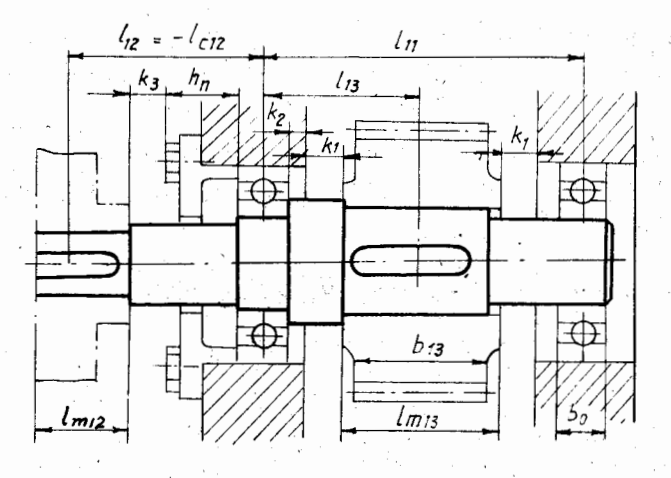
\includegraphics[width=150mm]{shaft1.png}
	\caption{Shaft design and its dimensions}
	\label{shaft}
\end{figure}

In this section, we will find all the parameters in Figure \ref{shaft}. However, if a parameter has 2 numeric subscripts, the first one will denote the ordinal number of shafts.\\
Using equation (10.10), the gear hubs are $ l_{m13} = l_{m12} = 1.5d_1 =  45\unit{(mm)} $, $ l_{m23} = l_{m22} = 1.5d_2 = 52.5\unit{(mm)} $, where $ l_{m22} $ is the chain hub.\\
From table (10.3), we choose $ k_1=10\unit{(mm)}$, $ k_2=8\unit{(mm)} $, $ k_3=15\unit{(mm)} $, $ h_n=18\unit{(mm)} $. This parameters apply for both shafts in the system.\\
Table (10.4) introduces the formulas for several types of gearbox. Since our system only concerns about 1-level gear reducer, the ones below are used:\\
On shaft 1:\\
$ l_{12} = -l_{c12} = -\left[ 0.5(l_{m12}+b_{O1})+k_3+h_n  \right] = -65 \unit{(mm)} $\\
$ l_{13} = 0.5(l_{m13}+b_{O1})+k_1+k_2 = 50 \unit{(mm)} $\\
$ l_{11} = 2l_{13} = 100 \unit{(mm)}$\\
On shaft 2:\\
$ l_{22} = -l_{c22} = -\left[ 0.5(l_{m22}+b_{O2})+k_3+h_n \right] = -69.75 \unit{(mm)} $\\
$ l_{23} = 0.5(l_{m23}+b_{O2})+k_1+k_2 = 54.75 \unit{(mm)} $\\
$ l_{21} = 2l_{23} = 109.5 \unit{(mm)}$


\subsection{Determine shaft diameters and lengths}

\paragraph{Find reaction forces}

\begin{figure}[ht]
	\centering
	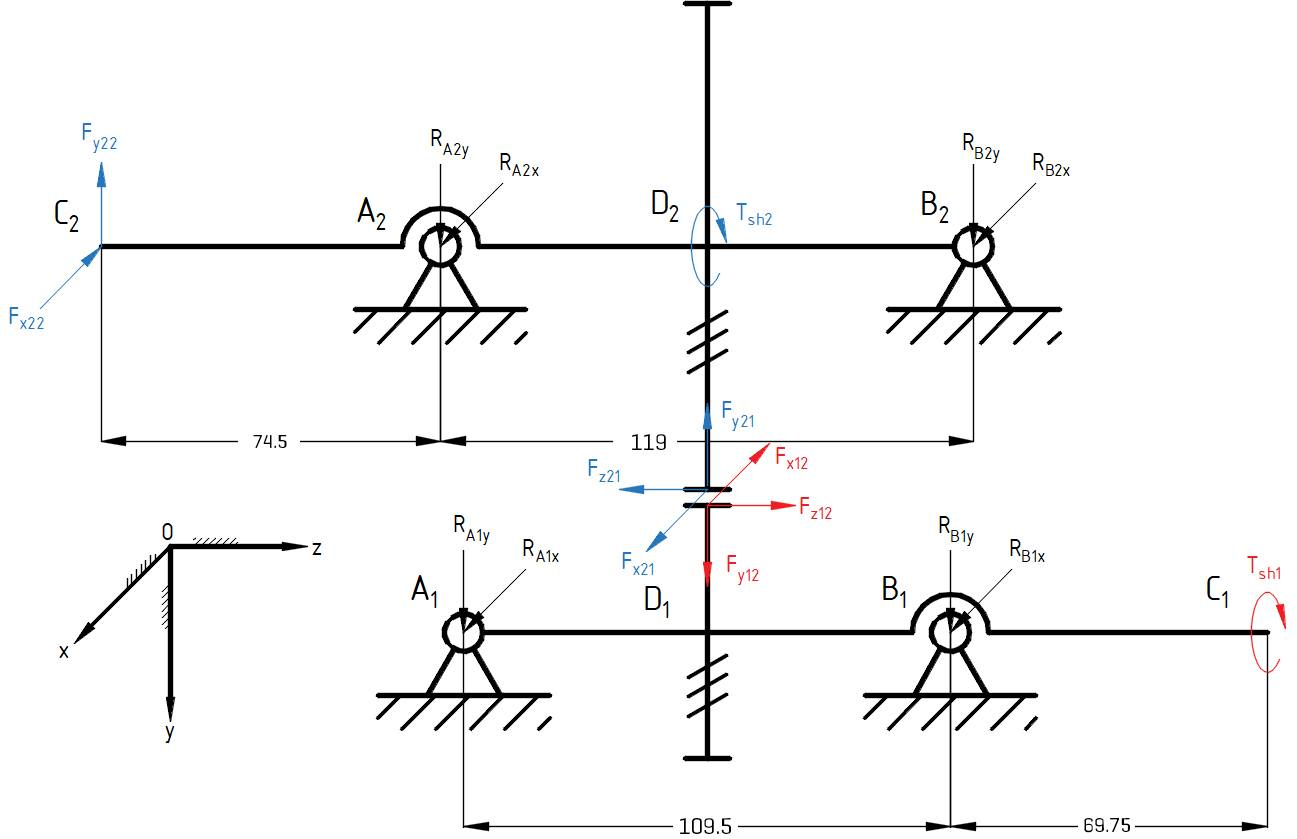
\includegraphics[width=160mm]{shaft.png}
	\caption{Force analysis of 2 shafts}
	\label{force on shaft}
\end{figure}

From the diagram, we solve for the reaction forces at $ A_1 $, $ A_2 $, $ B_1 $, $ B_2 $, which are $ R_{A1x} $, $ R_{A1y} $, $ R_{B1x} $, $ R_{B1y} $, $ R_{A2x} $, $ R_{A2y} $, $ R_{B2x} $, $ R_{B2y} $. Using equilibrium conditions
\[
\left\{ 
\begin{array}{l@{{}={}}l}
\displaystyle\sum_{i} \mathbf{F_{i}} & 0\\
\displaystyle\sum_{i} \mathbf{r_i}\times \mathbf{F_i}& 0\\
\end{array}
\right.
\]
we obtain the results:\vskip2mm
%\begin{table}[ht]
	{\centering
	\begin{tabular}[ht]{p{7cm}p{7cm}}
		$
		\left\{ 
		\begin{array}{l@{{} \approx {}}l}
		R_{A1x} & 1501.58\unit{(N)}\\
		R_{A1y} & -945.25\unit{(N)}\\
		R_{B1x} & 1501.58\unit{(N)}\\
		R_{B1y} & -252.42\unit{(N)}\\
		\end{array}
		\right.
		$ & $
		\left\{ 
		\begin{array}{l@{{} \approx {}}l}
		R_{A2x} & 691.13\unit{(N)}\\
		R_{A2y} & 2814.73\unit{(N)}\\
		R_{B2x} & -2354.81\unit{(N)}\\
		R_{B2y} & 702.99\unit{(N)}\\
		\end{array}
		\right.
		$
	\end{tabular}}
%\end{table}

\paragraph{Draw bending moment - torque diagrams} Knowing the reaction forces, we can easily draw bending moment and torque diagram for both shafts on 2 major planes (xOz) and (yOz).

\begin{figure}[ht]
	\centering
	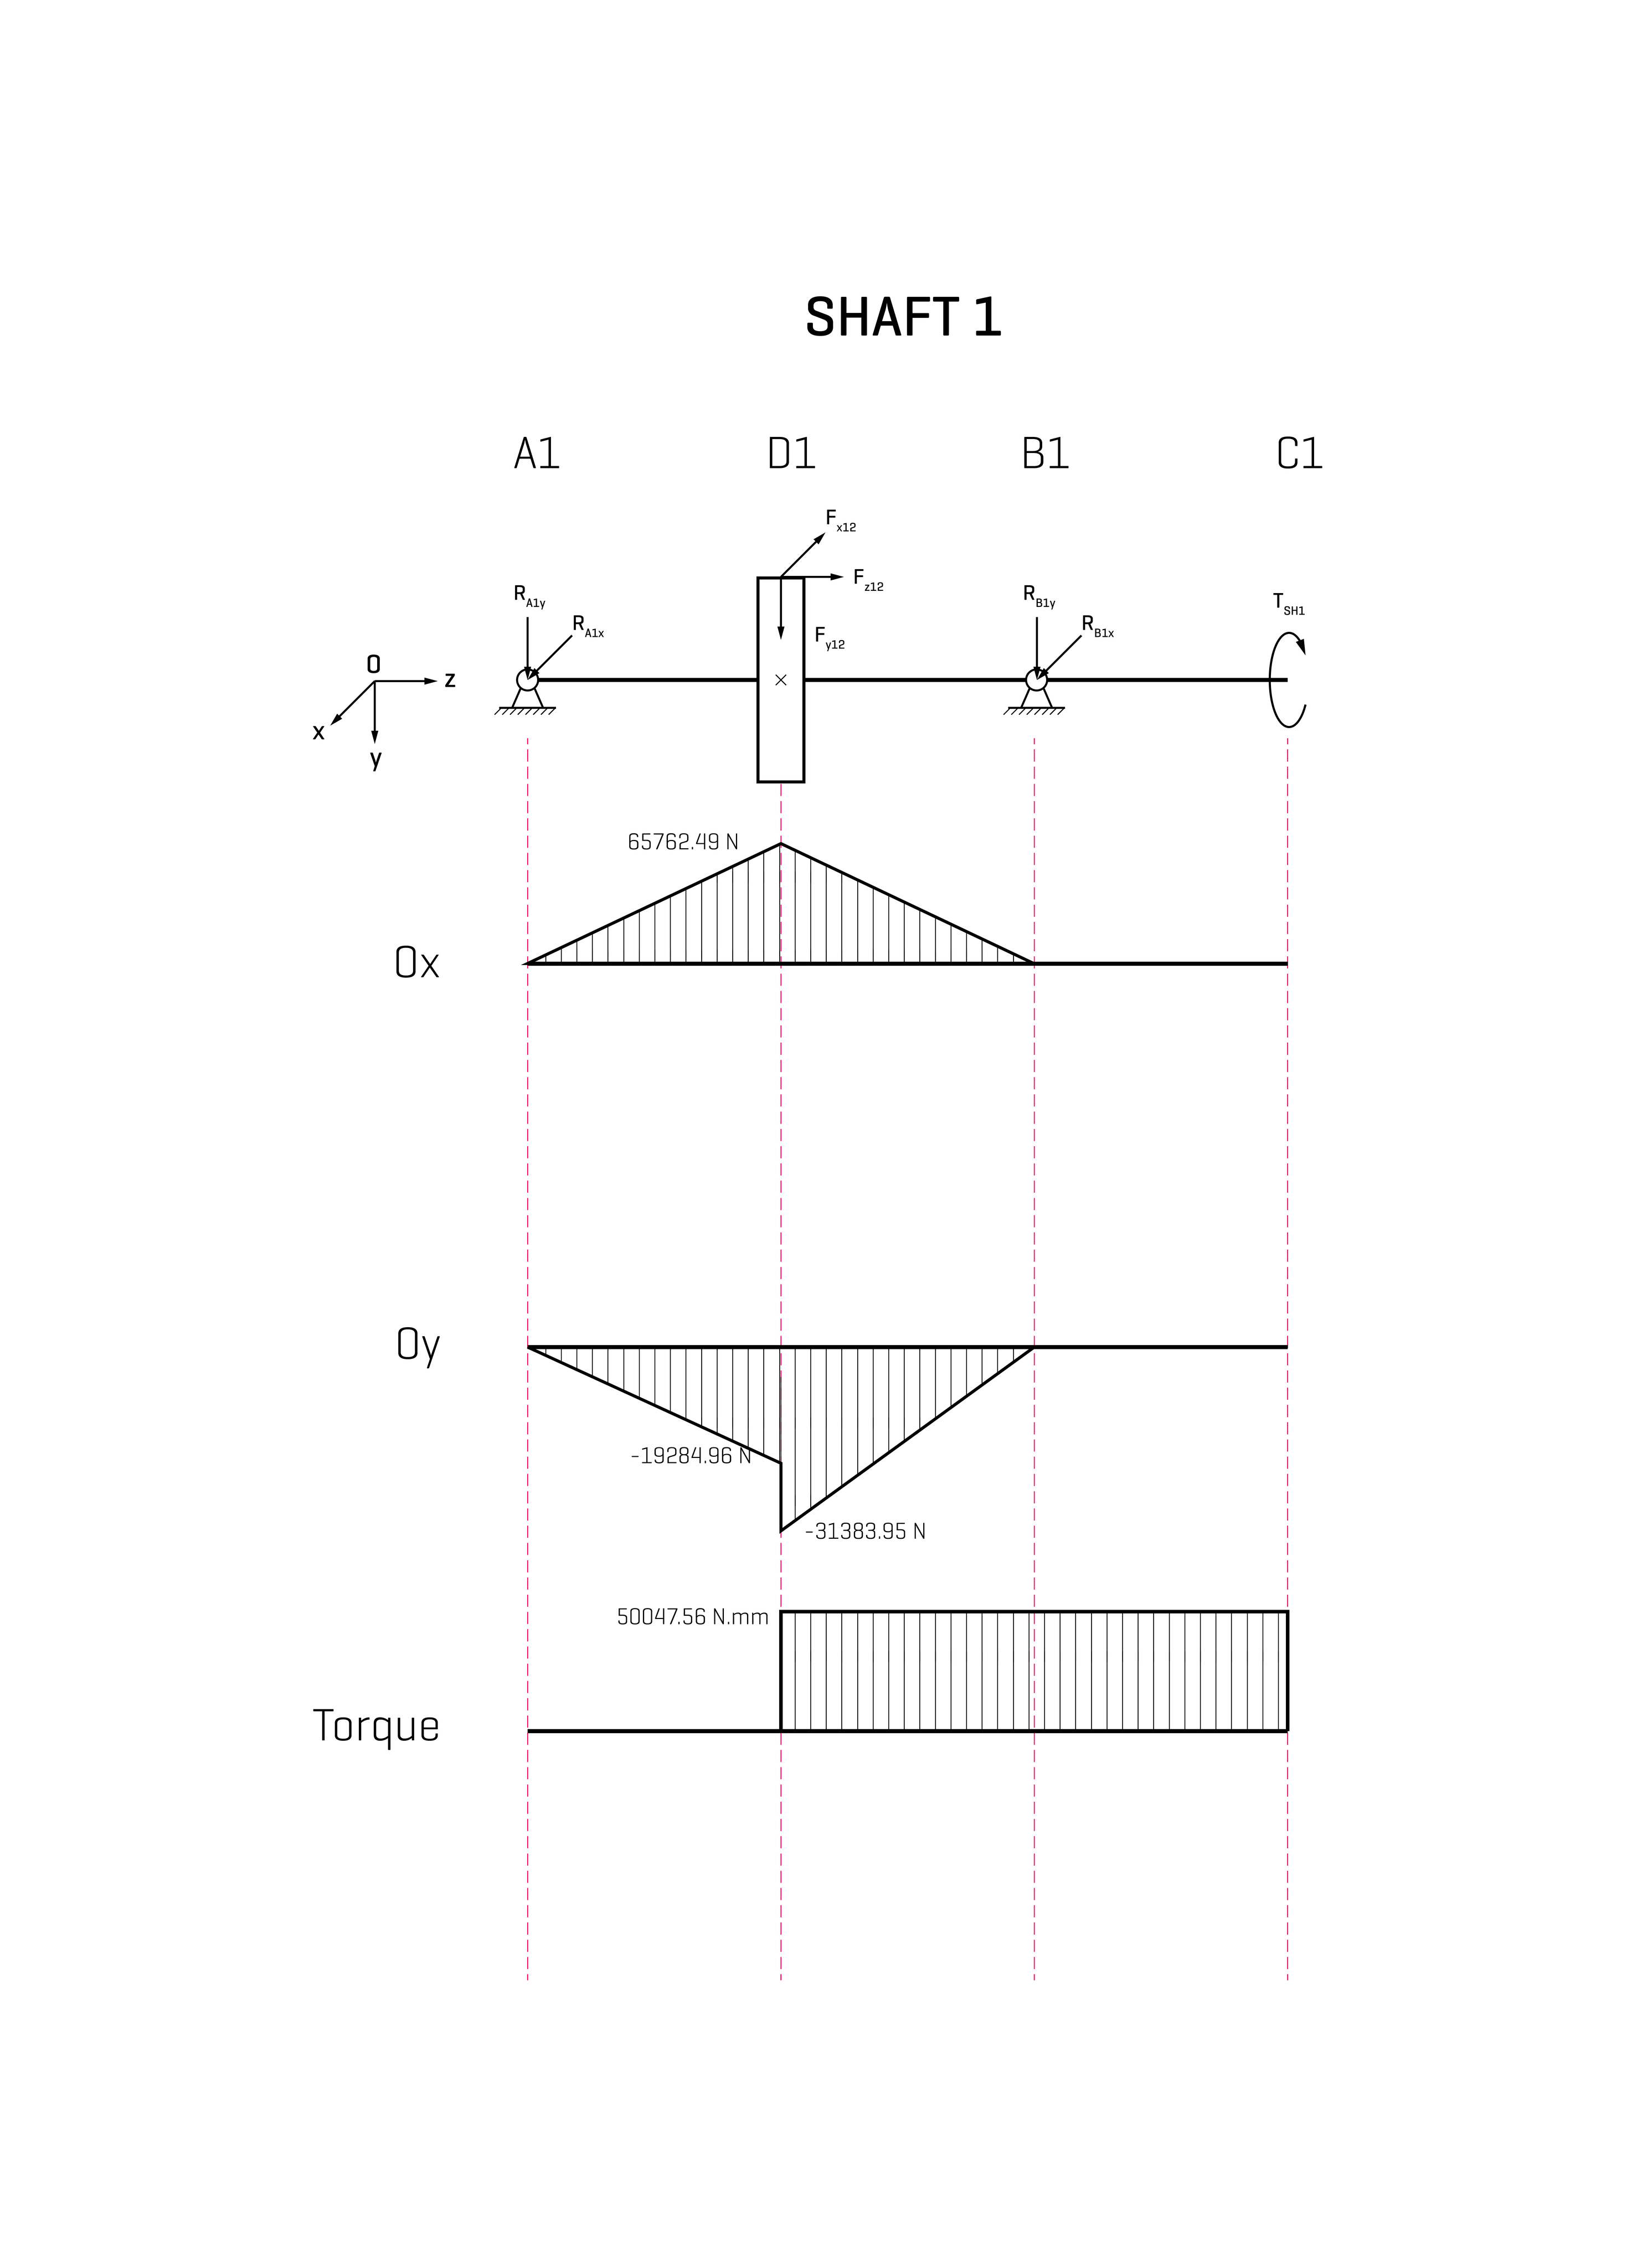
\includegraphics[width=160mm]{mshaft1.png}
	\caption{Bending moment-torque diagram of shaft 1}
	\label{mshaft1}
\end{figure}

\begin{figure}[ht]
	\centering
	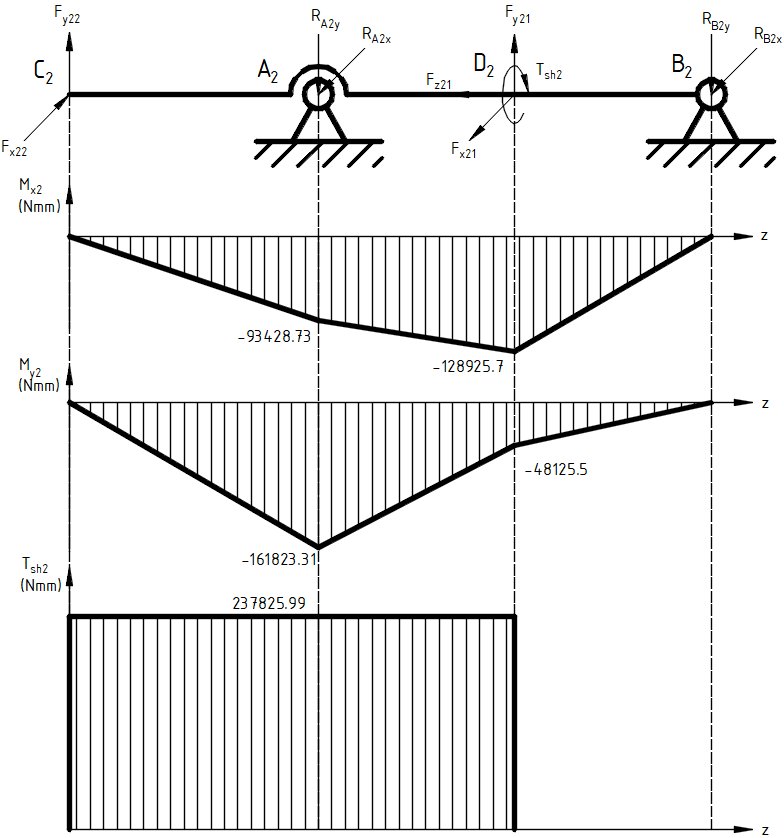
\includegraphics[width=153mm]{mshaft2.png}
	\caption{Bending moment-torque diagram of shaft 2}
	\label{mshaft2}
\end{figure}

\paragraph{Find equivalent moments} Knowing $ T_{sh1} $ and $ T_{sh2} $, we calculate equivalent moment $ M_e $ at the 8 points specified using the formula below:
\[M_e = \sqrt{M_x^2 + M_y^2 + 0.75T_{sh}^2}\]

%\begin{table}[ht]
%	\centering
	\begin{tabular}{p{7cm}p{7cm}}
		$
		\left\{ 
		\begin{array}{l@{{} \approx {}}l}
		M_{eA1} & 43342.4\unit{(N\cdot mm)}\\
		M_{eD1} & 91716.45\unit{(N\cdot mm)}\\
		M_{eB1} & 43342.46\unit{(N\cdot mm)}\\
		M_{eC1} & 43342.46\unit{(N\cdot mm)}\\
		\end{array}
		\right.
		$ &
		$
		\left\{ 
		\begin{array}{l@{{} \approx {}}l}
		M_{eC2} & 205963.35\unit{(N\cdot mm)}\\
		M_{eA2} & 278094.61\unit{(N\cdot mm)}\\
		M_{eD2} & 247707.09\unit{(N\cdot mm)}\\
		M_{eB2} & 205963.35\unit{(N\cdot mm)}\\
		\end{array}
		\right.
		$
	\end{tabular}\vskip2mm
%\end{table}

\paragraph{Find permissible stress}
$ [\sigma_1] $ and $ [\sigma_2] $ are determined by table (10.5). Since we use quenched 45X steel, $ [\sigma_1] = 67 \unit{(MPa)}$ and $ [\sigma_2] = 64 \unit{(MPa)}$ ($ [\sigma_2] $ is achieved using interpolation).

\paragraph{Find standardized diameters at specific locations on the shaft} Having $ M_e $ and $ [\sigma] $, the next step is to estimate specific diameter at the key points mentioned above using this formula, which only applies for rigid shafts:
\[d = \sqrt[3]{\dfrac{M_e}{0.1[\sigma]}}\]

\begin{tabular}{p{7cm}p{7cm}}
		$
		\left\{ 
		\begin{array}{l@{{} \approx {}}l}
		d_{A1} & 18.63 \unit{(mm)}\\
		d_{D1} & 23.92 \unit{(mm)}\\
		d_{B1} & 18.63 \unit{(mm)}\\
		d_{C1} & 18.63 \unit{(mm)}\\
		\end{array}
		\right.
		$ &
		$
		\left\{ 
		\begin{array}{l@{{} \approx {}}l}
		d_{C2} & 31.81 \unit{(mm)}\\
		d_{A2} & 35.16 \unit{(mm)}\\
		d_{D2} & 33.83 \unit{(mm)}\\
		d_{B2} & 31.81\unit{(mm)}\\
		\end{array}
		\right.
		$
	\end{tabular}

After rough calculations, we will choose the diameters based on standards (one applies for bearings while the other is used for the remaining machine elements), which is given on p.195:

	\begin{tabular}{p{7cm}p{7cm}}
		$
		\left\{ 
		\begin{array}{l@{{} = {}}l}
		d_{A1} & 20 \unit{(mm)}\\
		d_{D1} & 24 \unit{(mm)}\\
		d_{B1} & 20 \unit{(mm)}\\
		d_{C1} & 19 \unit{(mm)}\\
		\end{array}
		\right.
		$ &
		$
		\left\{ 
		\begin{array}{l@{{} = {}}l}
		d_{C2} & 32 \unit{(mm)}\\
		d_{A2} & 40 \unit{(mm)}\\
		d_{D2} & 34 \unit{(mm)}\\
		d_{B2} & 35 \unit{(mm)}\\
		\end{array}
		\right.
		$
	\end{tabular}

\section{Fatigue Strength Analysis}
For each critical point, the fatigue strength there must satisfy this condition:
\[s=\dfrac{s_\sigma s_\tau}{\sqrt{s_\sigma^2+s_\tau^2}}\geq[s]\]
\paragraph{Find $ K_{\sigma} $} 
%\paragraph{Find $ a_w $} On p.149, the following formula is used:
%\begin{equation}
%	a_w = (z_2+q)\sqrt[3]{\left( \dfrac{170}{z_2[\sigma_H]}\right) ^2 \dfrac{T_2K_H}{q}}
%\end{equation}